\chapter{التناظر والزمر النقطية}\label{ch:b3:point-groups}

أدِر ندفة ثلج ستين درجة فلا يتغير شيء؛ وأدِر جزيء
بنزين بالزاوية نفسها، فتقع ذرات الكربون الست وذرات الهيدروجين الست
تمامًا في مواضع بعضها. يحدد تناظر الجزيء عددًا من
خواصه قبل أي حساب: هل يمكن أن يكون له عزم ثنائي
قطب، وهل يمكن أن يوجد في صورتين هما خيالان مرآويان، وأي
اهتزازاته يمتص الأشعة تحت الحمراء، وأي المدارات يمكن أن يمتزج. ولاستعماله
استعار الكيميائيون من الرياضيات لغة الزمر. يعرّف هذا الفصل
\omterm{def:b3:point-groups:operation}{عمليات التناظر} في الجزيء، ويجمعها في \omterm{def:b3:point-groups:point-group}{زمرته النقطية}،
ويعطي إجراءً لإيجاد هذه الزمرة، ويبرهن مبرهنتين في القطبية
والكيرالية، ويقدّم \omterm{def:b3:point-groups:irrep}{جداول المميِّزات} التي يبني عليها
\cref{ch:b3:group-theory-applied}.

\begin{recall}
تنبأ مجلد السنة الأولى بأشكال الجزيئات بنموذج VSEPR، وعرّف
عزم ثنائي القطب للجزيء القطبي، وعرّف الكيرالية: فالجزيء الكيرالي
لا يمكن أن ينطبق على خياله المرآوي. واستعمل مجلد السنة الثانية
التناظر بالكلمات لبناء مدارات الشظايا للجزيئين \ce{H2O} و\ce{NH3}.
\end{recall}

\begin{omfigure}
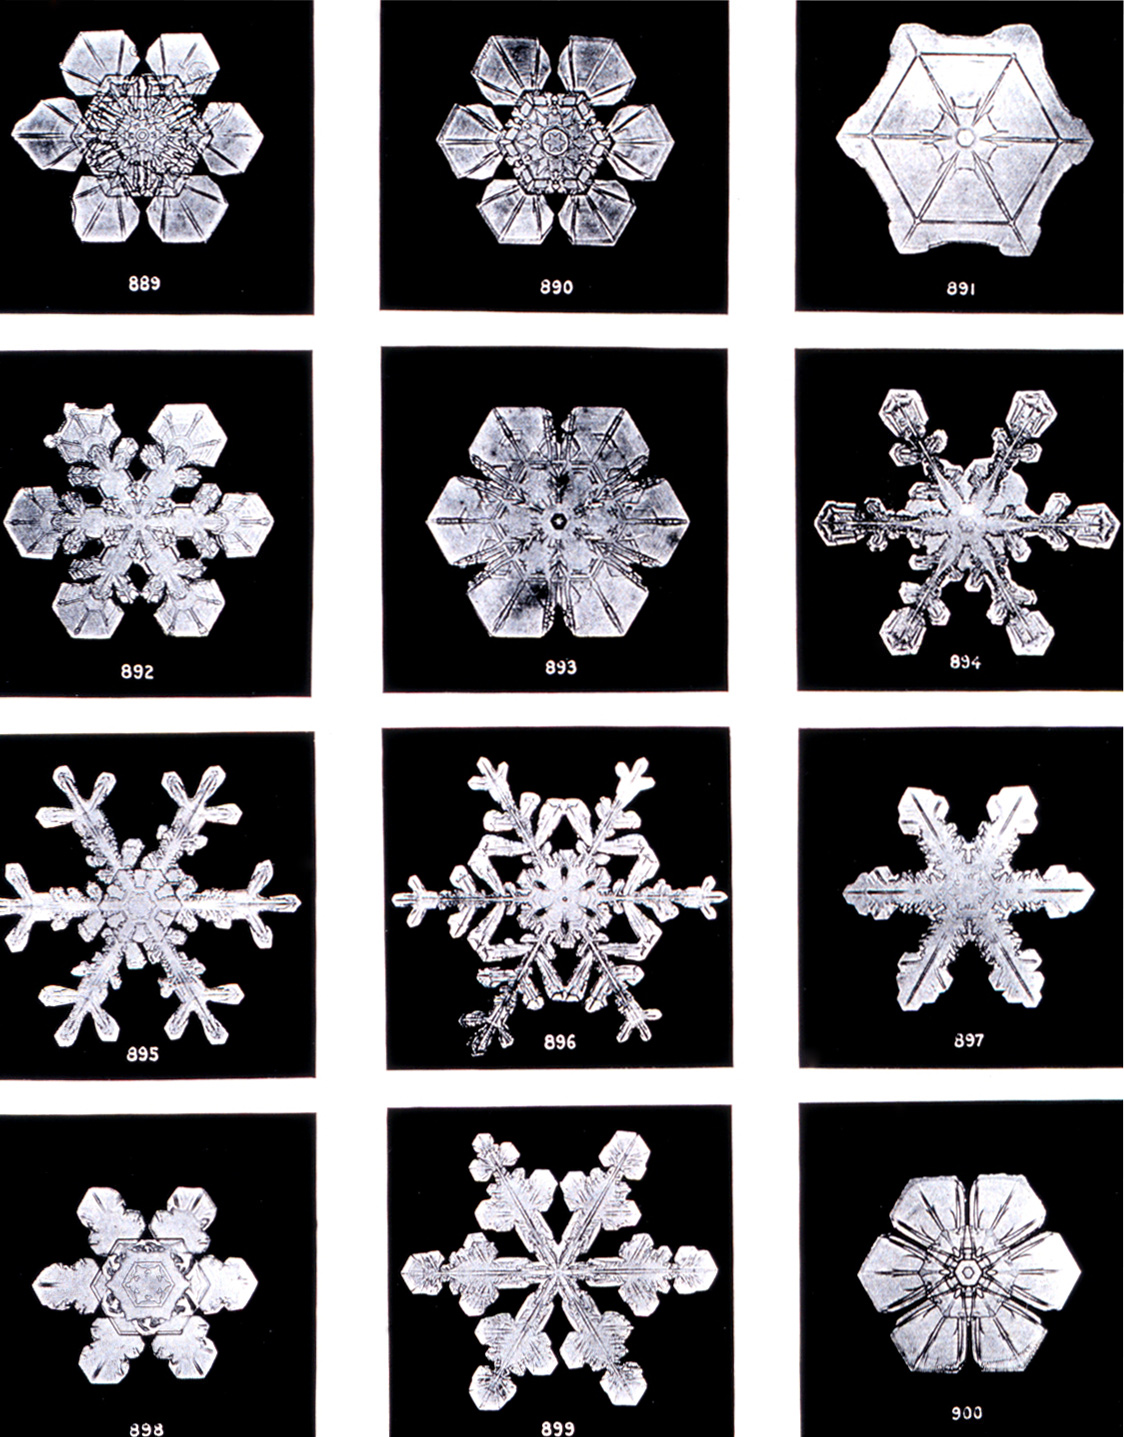
\includegraphics[width=0.4\linewidth]{images/book4/bentley-snowflakes.jpg}\hspace{1em}%
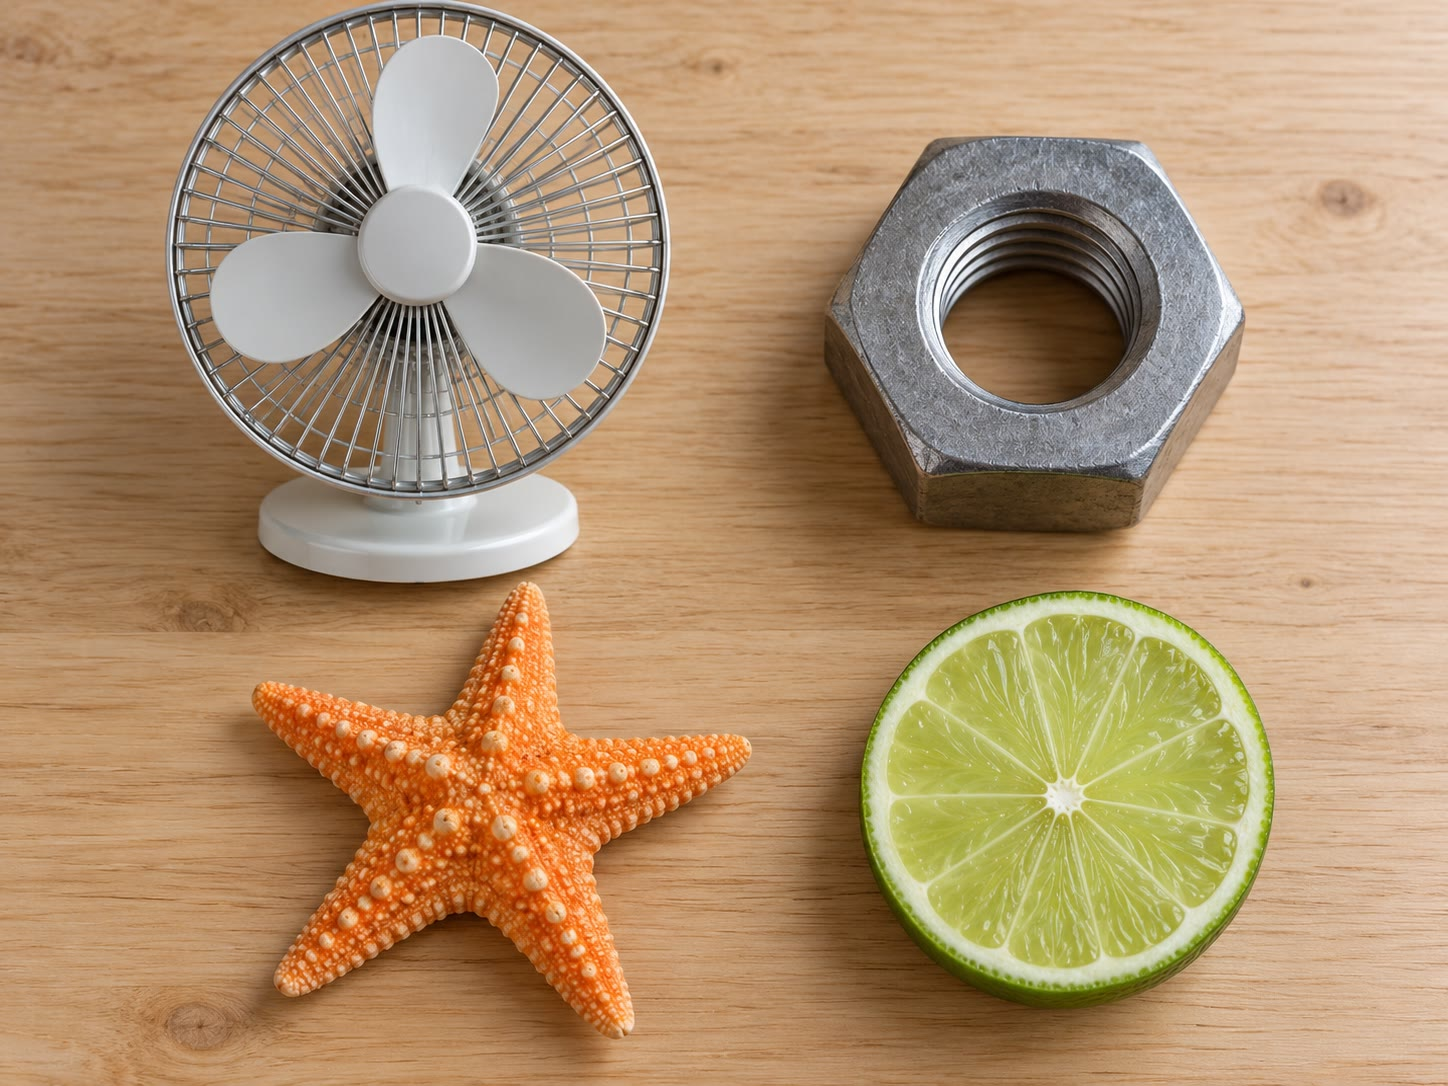
\includegraphics[width=0.48\linewidth]{images/book4/ai/b3-04-symmetric-objects.jpg}

{\small يسارًا: بلورات ثلج صوّرها ويلسون بنتلي نحو سنة 1902،
لكل منها تناظر سداسي. يمينًا: أشياء يومية ذات تناظر دوراني ثلاثي وسداسي
وخماسي.}
\end{omfigure}

\section{عمليات التناظر وعناصره}

\begin{definition}[عملية التناظر، عنصر التناظر]\label{def:b3:point-groups:operation}
\emph{عملية التناظر}\index{عملية تناظر} حركة أو
انعكاس يترك الجزيء في ترتيب لا يمكن تمييزه من
الترتيب الأصلي (كل ذرة في موضع كانت تشغله قبلًا ذرة من
النوع نفسه). و\emph{عنصر التناظر}\index{عنصر تناظر} هو الكائن
الهندسي --- نقطة أو مستقيم أو مستوٍ --- الذي تُجرى العملية
بالنسبة إليه.
\end{definition}

لكل جزيء العملية المحايدة $E$، التي لا تفعل شيئًا. أما
العمليات الأخرى فهي من أربعة أنواع.

\begin{definition}[محور الدوران الفعلي، المحور الرئيسي]\label{def:b3:point-groups:rotation}
\emph{محور الدوران الفعلي}\index{محور دوران فعلي} $C_n$ مستقيم
يكون الدوران حوله بزاوية $2\pi/n$ \omterm{def:b3:point-groups:operation}{عملية تناظر}، تُكتب أيضًا
$C_n$؛ وقواه $C_n^k$ دورانات بزاوية $2\pi k/n$، و$C_n^n = E$. 
والمحور ذو أعلى $n$ هو \emph{المحور الرئيسي}\index{محور رئيسي}، ويُتخذ
محورًا $z$.
\end{definition}

\begin{definition}[مستويات المرآة]\label{def:b3:point-groups:mirror}
\emph{مستوي المرآة}\index{مستوي مرآة} $\sigma$ مستوٍ يكون
الانعكاس فيه \omterm{def:b3:point-groups:operation}{عملية تناظر}؛ $\sigma^2 = E$. ويكون مستوي المرآة
\emph{مستوي مرآة رأسيًا}\index{مستوي مرآة رأسي} $\sigma_v$ إذا
احتوى \omterm{def:b3:point-groups:rotation}{المحور الرئيسي}، و\emph{مستوي مرآة
أفقيًا}\index{مستوي مرآة أفقي} $\sigma_h$ إذا كان عموديًا
عليه، و\emph{مستوي مرآة ثنائي الزاوية}\index{مستوي مرآة ثنائي الزاوية}
$\sigma_d$ إذا احتوى \omterm{def:b3:point-groups:rotation}{المحور الرئيسي} ونصّف الزاوية بين
محورين $C_2$ عموديين عليه.
\end{definition}

\begin{definition}[مركز الانقلاب]\label{def:b3:point-groups:inversion}
\emph{مركز الانقلاب}\index{مركز انقلاب} $i$ نقطة يكون
الانقلاب بالنسبة إليها، $(x, y, z) \mapsto (-x, -y, -z)$، \omterm{def:b3:point-groups:operation}{عملية
تناظر}.
\end{definition}

\begin{definition}[محور الدوران غير الفعلي]\label{def:b3:point-groups:improper}
\emph{محور الدوران غير الفعلي}\index{محور دوران غير فعلي} $S_n$
مستقيم يكون الدوران حوله بزاوية $2\pi/n$ متبوعًا بالانعكاس في المستوي
العمودي عليه \omterm{def:b3:point-groups:operation}{عملية تناظر}. و$S_1 = \sigma$ و$S_2 = i$.
\end{definition}

\begin{example}[عناصر أربعة جزيئات]\label{ex:b3:point-groups:elements}
\ce{H2O}: $E$، ومحور $C_2$ ينصّف الزاوية H--O--H، ومستويان
رأسيان، مستوي الجزيء والمستوي العمودي عليه. \ce{NH3}:
$E$، ومحور $C_3$ يمر بالذرة N (العمليتان $C_3$ و$C_3^2$)، وثلاثة مستويات $\sigma_v$، يحتوي كل منها
رابطة N--H واحدة. \ce{BF3}: محور $C_3$، وثلاثة محاور $C_2$ على امتداد الروابط B--F،
و$\sigma_h$ (مستوي الجزيء)، وثلاثة مستويات $\sigma_v$، ومحور $S_3$. \ce{CH4}: أربعة محاور
$C_3$ على امتداد الروابط C--H، وثلاثة محاور $C_2$ تنصّف الزوايا H--C--H، وهي
أيضًا محاور $S_4$، وستة مستويات $\sigma_d$، يحتوي كل منها رابطتين C--H
(الشكل أدناه).
\end{example}

\begin{omfigure}
\begin{tikzpicture}[font=\small]
  % H2O, side view: molecular plane xz (shaded), C2 along z
  \begin{scope}
    \fill[omDef!10] (-1.5,-1.0) -- (1.5,-1.0) -- (1.5,1.2) -- (-1.5,1.2) -- cycle;
    \fill[omThm!12, opacity=0.8] (-0.45,-1.35) -- (0.45,-0.65) -- (0.45,1.55) -- (-0.45,0.85) -- cycle;
    \draw[densely dashed, black!70] (0,-1.4) -- (0,1.7) node[above] {$C_2$};
    \node[aO] (o) at (0,0.5) {};
    \node[aH] (h1) at (-0.95,-0.25) {};
    \node[aH] (h2) at (0.95,-0.25) {};
    \begin{scope}[on background layer]
      \draw[bond] (o.center) -- (h1.center) (o.center) -- (h2.center);
    \end{scope}
    \node[omDef, anchor=north west] at (-1.5,1.2) {$\sigma_v(xz)$};
    \node[omThm, anchor=west] at (0.5,-0.85) {$\sigma_v'(yz)$};
    \node[anchor=north] at (0,-1.6) {\ce{H2O}, $C_{2v}$};
  \end{scope}
  % NH3, top view along C3
  \begin{scope}[xshift=4.0cm]
    \foreach \a in {90,210,330}{\draw[ommirror] (0,0) -- (\a:1.35); \draw[ommirror, black!40] (0,0) -- (\a+180:1.0);}
    \foreach \a in {90,210,330}{\node[aH] at (\a:0.95) {};}
    \node[aN] at (0,0) {};
    \pic at (0,0) {omthreefold};
    \node[anchor=north] at (0,-1.6) {\foreignlanguage{arabic}{\ce{NH3}، $C_{3v}$، منظورًا من أعلى}};
  \end{scope}
  % BF3, top view; sigma_h = plane of the paper (thick circle)
  \begin{scope}[xshift=8.0cm]
    \draw[ommirror] (0,0) circle (1.3);
    \foreach \a in {90,210,330}{\draw[ommirror] (\a:1.3) -- (\a+180:1.3);}
    \foreach \a in {90,210,330}{\pic[rotate=\a-90] at (\a:1.42) {omtwofold}; \pic[rotate=\a-90] at (\a+180:1.42) {omtwofold};}
    \foreach \a in {90,210,330}{\node[aF] at (\a:0.95) {};}
    \node[aX={pink!70!gray}{5.6mm}] at (0,0) {};
    \pic at (0,0) {omthreefold};
    \node[anchor=north] at (0,-1.6) {\foreignlanguage{arabic}{\ce{BF3}، $D_{3h}$، منظورًا من أعلى}};
  \end{scope}
\end{tikzpicture}

{\small \omterm{def:b3:point-groups:operation}{عناصر التناظر}. \ce{H2O}: المحور $C_2$ (متقطع) ومستويا المرآة
الرأسيان. \ce{NH3} و\ce{BF3} منظورًا إليهما على امتداد محورهما الرئيسي (رمز
المثلث): الخطوط الثخينة مستويات مرآة منظور إليها من حافتها؛ وفي \ce{BF3} تدل الدائرة
الثخينة على \omterm{def:b3:point-groups:mirror}{مستوي المرآة الأفقي} (مستوي الصفحة) ورموز
العدسة على محاور $C_2$ الثلاثة الواقعة فيه.}
\end{omfigure}

\section{الزمر}

\begin{proposition}[جداءات عمليات التناظر]\label{prop:b3:point-groups:closure}
إجراء عمليتي تناظر لجزيء على التوالي \omterm{def:b3:point-groups:operation}{عملية تناظر}
لذلك الجزيء أيضًا. ومع $E$ ومقلوب
كل عملية، تشكّل مجموعة \omterm{def:b3:point-groups:operation}{عمليات التناظر} زمرة: جداء تجميعي،
وعنصر محايد، ومقلوب لكل عنصر.
\end{proposition}

\begin{proof}
كل عملية تترك الجزيء غير قابل للتمييز من نفسه، وكذلك عمليتان
متتاليتان. وجداء العمليات (تركيب تطبيقات الفضاء)
تجميعي؛ و$E$ العنصر المحايد؛ والعملية المعكوسة (دوران بالزاوية
المعاكسة، أو انعكاس مكرَّر) \omterm{def:b3:point-groups:operation}{عملية تناظر} أيضًا.
\end{proof}

\begin{proposition}[نقطة مشتركة]\label{prop:b3:point-groups:fixed-point}
تمر كل \omterm{def:b3:point-groups:operation}{عناصر التناظر} لجزيء منته بنقطة واحدة.
\end{proposition}

\begin{proof}
كل \omterm{def:b3:point-groups:operation}{عملية تناظر} تنقل كل ذرة إلى ذرة لها الكتلة نفسها، فهي
تترك مركز الكتلة دون تغيير. والدوران لا يثبّت إلا نقاط
محوره، والانعكاس نقاط مستويه، والدوران غير الفعلي أو الانقلاب
نقطة واحدة: فكل عنصر يحتوي مركز الكتلة.
\end{proof}

\begin{definition}[الزمرة النقطية، رتبة الزمرة النقطية]\label{def:b3:point-groups:point-group}
زمرة كل \omterm{def:b3:point-groups:operation}{عمليات التناظر} لجزيء هي \emph{زمرته
النقطية}\index{زمرة نقطية}، وسُمّيت كذلك لأن نقطة واحدة تبقى ثابتة. وعدد
عملياتها هو \emph{رتبة الزمرة النقطية}\index{رتبة الزمرة النقطية}،
$h$.
\end{definition}

\begin{example}[زمرة الماء]\label{ex:b3:point-groups:c2v}
العمليات الأربع $E$ و$C_2$ و$\sigma_v(xz)$ و$\sigma_v'(yz)$ للجزيء \ce{H2O} تشكّل
زمرة رتبتها 4. وجدول ضربها (عملية السطر تُجرى بعد عملية
العمود) هو
\begin{center}\small
\begin{tabular}{c|cccc}
\hline
 & $E$ & $C_2$ & $\sigma_v(xz)$ & $\sigma_v'(yz)$\\ \hline
$E$ & $E$ & $C_2$ & $\sigma_v(xz)$ & $\sigma_v'(yz)$\\
$C_2$ & $C_2$ & $E$ & $\sigma_v'(yz)$ & $\sigma_v(xz)$\\
$\sigma_v(xz)$ & $\sigma_v(xz)$ & $\sigma_v'(yz)$ & $E$ & $C_2$\\
$\sigma_v'(yz)$ & $\sigma_v'(yz)$ & $\sigma_v(xz)$ & $C_2$ & $E$\\ \hline
\end{tabular}
\end{center}
فمثلًا تنتقل نقطة $(x, y, z)$ منعكسة في $xz$ إلى $(x, -y, z)$، ثم
بالدوران بزاوية $\pi$ حول $z$ إلى $(-x, y, z)$: وهذا هو نفسه انعكاس واحد في
$yz$.
\end{example}

\begin{definition}[صنف عمليات التناظر، الزمرة الجزئية]\label{def:b3:point-groups:class}
تنتمي عمليتان $A$ و$B$ إلى \emph{صنف عمليات
التناظر}\index{صنف عمليات التناظر} نفسه إذا كان $B = X^{-1}AX$ من أجل
عملية ما $X$ من الزمرة: فهما من نوع العملية نفسه، منظورًا إليه في
معلم حرّكته $X$. والمجموعة الجزئية من زمرة التي هي زمرة بذاتها
\emph{زمرة جزئية}\index{زمرة جزئية}؛ ورتبتها تقسم رتبة الزمرة.
\end{definition}

\begin{example}[أصناف \ce{NH3}]\label{ex:b3:point-groups:classes}
في $C_{3v}$ ($h = 6$)، تشكّل الانعكاسات الثلاثة صنفًا واحدًا (فالدوران $C_3$
ينقل كل مستوٍ إلى آخر)، والدورانان $C_3$ و$C_3^2$ صنفًا آخر،
و$E$ صنف وحده: ثلاثة أصناف، تُكتب $E$ و$2C_3$ و$3\sigma_v$. وفي
$C_{2v}$ كل عملية صنف بمفردها: إذ لا عملية تحوّل أحد المستويين إلى
الآخر.
\end{example}

\begin{definition}[رمز شونفليس]\label{def:b3:point-groups:schoenflies}
تُسمى \omterm{def:b3:point-groups:point-group}{الزمرة النقطية} \emph{برمز شونفليس}\index{رمز شونفليس} الخاص بها:
$C_n$ (محور $C_n$ واحد)، و$C_{nv}$ (بإضافة $n$ مستويًا رأسيًا)، و$C_{nh}$
(بإضافة $\sigma_h$)، و$D_n$ (بإضافة $n$ محورًا $C_2$ عموديًا على $C_n$)، و$D_{nh}$
و$D_{nd}$ (بإضافة $\sigma_h$، أو $n$ مستويًا ثنائي الزاوية، إلى $D_n$)، و$S_{2n}$، 
والزمر المكعبية $T_d$ و$O_h$ و$I_h$ لرباعي الأوجه وثماني الأوجه
وعشريني الأوجه، و$C_s$ و$C_i$ و$C_1$ للجزيئات التي ليس لها إلا \omterm{def:b3:point-groups:mirror}{مستوي مرآة}،
أو إلا \omterm{def:b3:point-groups:inversion}{مركز انقلاب}، أو لا شيء البتة. وتنتمي الجزيئات الخطية إلى
$C_{\infty v}$ أو $D_{\infty h}$.
\end{definition}

\section{تعيين الزمرة النقطية}

\begin{method}[إيجاد الزمرة النقطية لجزيء]\label{met:b3:point-groups:assign}
\begin{enumerate}
  \item هل الجزيء خطي؟ إن كان له \omterm{def:b3:point-groups:inversion}{مركز انقلاب}، فزمرته $D_{\infty h}$
        (\ce{CO2}، \ce{N2})؛ وإلا فزمرته $C_{\infty v}$ (\ce{HCl}، \ce{HCN}).
  \item هل له عدة محاور من رتبة عالية ($n \ge 3$)؟ الشكل الرباعي الأوجه:
        $T_d$؛ الثماني الأوجه: $O_h$؛ العشريني الأوجه: $I_h$.
  \item جد \omterm{def:b3:point-groups:rotation}{المحور الرئيسي} $C_n$ (إن لم يوجد: $C_s$ إن وُجد مستوٍ، و$C_i$ إن وُجد
        مركز، و$C_1$ فيما عدا ذلك).
  \item هل توجد $n$ محاور $C_2$ عمودية على $C_n$؟ إن وُجدت فالزمرة
        $D_{nh}$ (مع $\sigma_h$)، وإلا $D_{nd}$ (مع $n$ مستويًا $\sigma_d$)، وإلا
        $D_n$.
  \item إن لم توجد: $C_{nh}$ (مع $\sigma_h$)، أو $C_{nv}$ (مع $n$ مستويًا $\sigma_v$)، أو $S_{2n}$
        (مع محور $S_{2n}$ وحده منطبق على $C_n$)، وإلا $C_n$.
\end{enumerate}
\end{method}

\begin{omfigure}
\begin{tikzpicture}[font=\footnotesize, node distance=6mm and 11mm,
  q/.style={draw=black!60, fill=omDef!6, rounded corners=2pt, align=center, inner sep=3pt},
  g/.style={draw=black!60, fill=omProp!10, rounded corners=2pt, inner sep=3pt}]
  \node[q] (lin) {\foreignlanguage{arabic}{خطي؟}};
  \node[g, right=of lin] (dinf) {\shortstack{\foreignlanguage{arabic}{$D_{\infty h}$ / $C_{\infty v}$ (مع $i$ / دونه)}}};
  \node[q, below=of lin] (cub) {\foreignlanguage{arabic}{محوران $C_n$ أو أكثر، $n \ge 3$؟}};
  \node[g, right=of cub] (td) {$T_d$, $O_h$, $I_h$};
  \node[q, below=of cub] (cn) {\foreignlanguage{arabic}{محور $C_n$؟}};
  \node[g, right=of cn] (low) {\shortstack{\foreignlanguage{arabic}{$C_s$ أو $C_i$ أو $C_1$ (لا محور)}}};
  \node[q, below=of cn] (c2) {\foreignlanguage{arabic}{$n$ محورًا $C_2 \perp C_n$؟}};
  \node[q, right=of c2, xshift=6mm] (dh) {\foreignlanguage{arabic}{$\sigma_h$؟\; وإلا $n$ مستويًا $\sigma_d$؟}};
  \node[g, right=of dh] (dg) {$D_{nh}$ / $D_{nd}$ / $D_n$};
  \node[q, below=of c2] (sh) {\foreignlanguage{arabic}{$\sigma_h$؟\; وإلا $n$ مستويًا $\sigma_v$؟\; وإلا $S_{2n}$؟}};
  \node[g, right=of sh] (cg) {$C_{nh}$ / $C_{nv}$ / $S_{2n}$ / $C_n$};
  \draw[->] (lin) -- node[above] {\foreignlanguage{arabic}{نعم}} (dinf);
  \draw[->] (lin) -- node[left] {\foreignlanguage{arabic}{لا}} (cub);
  \draw[->] (cub) -- node[above] {\foreignlanguage{arabic}{نعم}} (td);
  \draw[->] (cub) -- node[left] {\foreignlanguage{arabic}{لا}} (cn);
  \draw[->] (cn) -- node[above] {\foreignlanguage{arabic}{لا}} (low);
  \draw[->] (cn) -- node[left] {\foreignlanguage{arabic}{نعم}} (c2);
  \draw[->] (c2) -- node[above] {\foreignlanguage{arabic}{نعم}} (dh);
  \draw[->] (dh) -- (dg);
  \draw[->] (c2) -- node[left] {\foreignlanguage{arabic}{لا}} (sh);
  \draw[->] (sh) -- (cg);
\end{tikzpicture}

{\small البحث عن \omterm{def:b3:point-groups:point-group}{الزمرة النقطية}، بترتيب خطوات الطريقة.}
\end{omfigure}

\begin{example}[معرض]\label{ex:b3:point-groups:gallery}
\ce{H2O} و\ce{CH2Cl2} و\ce{SO2}: $C_{2v}$. \ce{NH3} و\ce{CHCl3}: $C_{3v}$. \ce{BF3}
و\ce{PCl5}: $D_{3h}$. \ce{CH4} و\ce{CCl4}: $T_d$. \ce{SF6}: $O_h$. البنزين: $D_{6h}$.
الإيثين: $D_{2h}$. الإيثان: $D_{3d}$ متخالفًا، و$D_{3h}$ متطابقًا. الألين
\ce{H2C=C=CH2}: $D_{2d}$، ومستويا المجموعتين \ce{CH2} متعامدان. والهكسان الحلقي
في تشكّل الكرسي: $D_{3d}$. trans-\ce{N2F2}: $C_{2h}$. \ce{CHFClBr}: $C_1$.
\end{example}

\begin{omfigure}
\tdplotsetmaincoords{60}{100}
\begin{tikzpicture}[tdplot_main_coords, scale=1.6, font=\small]
  \pic[transform shape] {omcubeo={2}};
  % depth order for view 60/100 (smallest first): H(0,0,0), H(0,2,2), C, H(2,2,0), H(2,0,2)
  \draw[densely dashed, omThm, thick] (-0.4,-0.4,-0.4) -- (2.5,2.5,2.5) node[anchor=south west] {$C_3$};
  \draw[densely dashed, omDef, thick] (1,1,-0.5) -- (1,1,2.6) node[anchor=south] {$S_4$, $C_2$};
  \node[aH] (h1) at (0,0,0) {};
  \node[aH] (h4) at (0,2,2) {};
  \node[aC] (c) at (1,1,1) {};
  \node[aH] (h2) at (2,2,0) {};
  \node[aH] (h3) at (2,0,2) {};
  \begin{scope}[on background layer]
    \draw[bond] (c.center) -- (h1.center) (c.center) -- (h2.center)
                (c.center) -- (h3.center) (c.center) -- (h4.center);
  \end{scope}
\end{tikzpicture}

{\small الميثان في مكعب، ذرة كربونه في المركز وذرات الهيدروجين على
رؤوس متناوبة. القطر الأكبر المار بذرة هيدروجين محور $C_3$
(وهي أربعة)؛ والمحور المار بمركزي وجهين متقابلين محور $C_2$ ومحور
$S_4$ (وهي ثلاثة). \omterm{def:b3:point-groups:point-group}{والزمرة النقطية} $T_d$، ورتبتها 24.}
\end{omfigure}

\section{النتائج: القطبية والكيرالية}

\begin{theorem}[الجزيئات القطبية]\label{thm:b3:point-groups:polar}
لا يمكن أن يكون لجزيء عزم ثنائي قطب دائم إلا إذا كانت \omterm{def:b3:point-groups:point-group}{زمرته النقطية}
$C_1$ أو $C_s$ أو $C_n$ أو $C_{nv}$؛ ويقع ثنائي القطب عندئذ على امتداد \omterm{def:b3:point-groups:rotation}{المحور الرئيسي}
(وفي المستوي، من أجل $C_s$).
\end{theorem}

\begin{proof}
عزم ثنائي القطب خاصية متجهية للجزيء، فيجب أن تتركه كل \omterm{def:b3:point-groups:operation}{عملية
تناظر} دون تغيير. والدوران حول محور لا يترك دون تغيير إلا
المتجهات الواقعة على هذا المحور؛ ومحوران لا يتركان أي متجهة غير معدومة؛ 
و$\sigma_h$ أو $i$ أو $S_n$ يعكس كل متجهة على امتداد المحور؛ و$\sigma_v$
يحفظ المتجهات الواقعة في مستويه. ومنه يقتضي ثنائي القطب غير المعدوم محورًا واحدًا على الأكثر،
ولا $\sigma_h$، ولا $i$، ولا $S_n$: وهي الزمر المذكورة.
\end{proof}

\begin{example}[قطبي أم لا]\label{ex:b3:point-groups:polar}
يمكن أن تكون \ce{H2O} و\ce{NH3} و\ce{CHCl3} و\ce{SO2} ($C_{2v}$، $C_{3v}$) قطبية، 
وهي كذلك فعلًا. أما \ce{BF3} ($D_{3h}$) و\ce{CO2} ($D_{\infty h}$) و\ce{CH4} ($T_d$) و\ce{SF6} ($O_h$)
وtrans-\ce{N2F2} ($C_{2h}$) فلا يمكن أن تكون كذلك، أيًا كانت قطبية روابطها.
\end{example}

\begin{theorem}[الجزيئات الكيرالية]\label{thm:b3:point-groups:chiral}
يكون الجزيء كيراليًا إذا وفقط إذا لم يكن له \omterm{def:b3:point-groups:improper}{محور دوران غير فعلي} $S_n$
(بما في ذلك $S_1 = \sigma$ و$S_2 = i$).
\end{theorem}

\begin{proof}
إذا كان للجزيء محور $S_n$، فإن $S_n = \sigma_hC_n$: الخيال المرآوي $\sigma_h$
للجزيء يساوي $C_n^{-1}$ مطبَّقًا على الجزيء بعد $S_n$، أي
الجزيء مدارًا --- فهو قابل للانطباق، ومنه لاكيرالي. وعكسيًا، إذا كان
الجزيء لاكيراليًا، أمكن نقل خياله المرآوي $\sigma M$ إلى $M$ بحركة
فعلية $R$ (دوران حول مركز الكتلة): فيكون $R\sigma$ عندئذ \omterm{def:b3:point-groups:operation}{عملية
تناظر}. وهي غير فعلية (تغيّر اليدوية، ومصفوفتها لها
المحدد $-1$)، وكل عملية غير فعلية في \omterm{def:b3:point-groups:point-group}{زمرة نقطية} هي
$S_n$ من أجل قيمة ما للعدد $n$ (دوران متبوع بانعكاس في المستوي
العمودي). فللجزيء إذن محور $S_n$.
\end{proof}

\begin{example}[جزيء لاكيرالي بلا مستوٍ]\label{ex:b3:point-groups:s4}
بعض الجزيئات ليس لها \omterm{def:b3:point-groups:mirror}{مستوي مرآة} ولا \omterm{def:b3:point-groups:inversion}{مركز انقلاب}، لكنها
لاكيرالية بسبب محور $S_4$: والحالة الكلاسيكية مركب سبيرو
مبني من حلقتين مستبدلتين بالطريقة نفسها ومتعامدتين، \omterm{def:b3:point-groups:point-group}{زمرته
النقطية} $S_4$. فلا يمكن الحكم على الكيرالية بالبحث عن مستوٍ وحده.
\end{example}

\section{التمثيلات وجداول المميِّزات}

كل \omterm{def:b3:point-groups:operation}{عملية تناظر} تنقل النقطة $(x, y, z)$ نقلًا خطيًا: فيمكن أن تُكتب
مصفوفةً $3\times3$.

\begin{definition}[التمثيل المصفوفي، المميِّز]\label{def:b3:point-groups:representation}
\emph{التمثيل المصفوفي}\index{تمثيل مصفوفي} $\Gamma$ \omterm{def:b3:point-groups:point-group}{لزمرة
نقطية} يقرن بكل عملية $R$ مصفوفة مربعة $D(R)$ بحيث
$D(R_1R_2) = D(R_1)D(R_2)$: فتصير جداءات العمليات جداءات
مصفوفات. و\emph{المميِّز}\index{مميِّز} $\chi(R)$ للعملية $R$ في $\Gamma$ هو
أثر $D(R)$.
\end{definition}

\begin{example}[إحداثيات $C_{3v}$]\label{ex:b3:point-groups:xyz}
من أجل $C_3$ حول $z$، $D = \begin{psmallmatrix}\cos120^\circ & -\sin120^\circ &
0\\ \sin120^\circ & \cos120^\circ & 0\\ 0 & 0 & 1\end{psmallmatrix}$، وأثرها
$2\cos120^\circ + 1 = 0$؛ ومن أجل $\sigma_v(xz)$، $D = \mathrm{diag}(1, -1, 1)$، وأثرها
1؛ ومن أجل $E$، الأثر 3. \omterm{def:b3:point-groups:representation}{فمميِّزات} هذا التمثيل هي $(3, 0, 1)$ على
الأصناف $(E, 2C_3, 3\sigma_v)$. وكل مصفوفة قطرية بالكتل، كتلة
$2\times2$ من أجل $(x, y)$ وكتلة $1\times1$ من أجل $z$: فالتمثيل
ينقسم إلى تمثيلين أصغر.
\end{example}

\begin{proposition}[المميِّزات دوال أصناف]\label{prop:b3:point-groups:class-characters}
للعمليات المنتمية إلى الصنف نفسه \omterm{def:b3:point-groups:representation}{المميِّز} نفسه في أي تمثيل.
\end{proposition}

\begin{proof}
إذا كان $B = X^{-1}AX$، فإن $D(B) = D(X)^{-1}D(A)D(X)$، والأثر لا يتغير بمثل
هذا التغيير للأساس: $\mathrm{tr}(P^{-1}MP) = \mathrm{tr}(M)$.
\end{proof}

\begin{proposition}[الاختزال بالكتل]\label{prop:b3:point-groups:direct-sum}
إذا أمكن تقسيم أساسٍ إلى مجموعات جزئية تنقل كل عملية كلًا منها إلى
نفسها، كانت كل المصفوفات قطرية بالكتل، وكان التمثيل
مجموع التمثيلات الأصغر التي تحملها المجموعات الجزئية؛ \omterm{def:b3:point-groups:representation}{ومميِّزاته}
مجاميع \omterm{def:b3:point-groups:representation}{مميِّزاتها}.
\end{proposition}

\begin{proof}
العملية التي تنقل كل مجموعة جزئية إلى نفسها ليس لها عناصر مصفوفة
بين مجموعات جزئية مختلفة؛ وأثر المصفوفة القطرية بالكتل مجموع
آثار كتلها.
\end{proof}

\begin{definition}[التمثيل غير القابل للاختزال، جدول المميِّزات، رمز موليكن]\label{def:b3:point-groups:irrep}
التمثيل الذي لا يمكن تقسيمه أكثر بأي تغيير للأساس
\emph{تمثيل غير قابل للاختزال}\index{تمثيل غير قابل للاختزال}. 
و\emph{جدول المميِّزات}\index{جدول المميِّزات} \omterm{def:b3:point-groups:point-group}{لزمرة نقطية} يسرد
\omterm{def:b3:point-groups:representation}{مميِّزات} تمثيلاتها غير القابلة للاختزال، سطرًا لكل منها، على أصنافها،
عمودًا لكل صنف، مع الدوال الديكارتية والدورانات التي تتحول
كما يتحول كل سطر. وتُسمى الأسطر \emph{برمز
موليكن}\index{رمز موليكن}: $A$ أو $B$ للبعد الواحد (متناظر أو
ضد متناظر بالدوران الرئيسي)، و$E$ للبعدين، و$T$ للثلاثة؛
والأدلة 1 و2 (متناظر أو ضد متناظر بمحور $C_2$ أو بمستوي $\sigma_v$)، و$g$ و$u$
(بالانقلاب)، والفتحات (بالمستوي $\sigma_h$).
\end{definition}

\begin{proposition}[حجم جدول المميِّزات]\label{prop:b3:point-groups:irrep-count}
\omterm{def:b3:point-groups:point-group}{للزمرة النقطية} من \omterm{def:b3:point-groups:irrep}{التمثيلات غير القابلة للاختزال} بقدر ما لها من أصناف، 
ومجموع مربعات أبعادها يساوي الرتبة: $\sum_id_i^2 = h$.
\end{proposition}
\begin{proof}[مكانتها]
تُبرهن في \cref{ch:b3:group-theory-applied} انطلاقًا من تعامد
\omterm{def:b3:point-groups:representation}{المميِّزات}، الذي يُقبل هناك دون برهان.
\end{proof}

% ledger: ct:C2v, ct:C3v, ct:Td
الجداول الأكثر استعمالًا في هذا الكتاب هي جداول الماء والأمونيا
والميثان:
\begin{omchartable}{C_{2v}}{cccc}{E & C_2 & \sigma_v(xz) & \sigma_v'(yz)}
A_1 & 1 & 1 & 1 & 1 & z & x^2,\ y^2,\ z^2 \\
A_2 & 1 & 1 & -1 & -1 & R_z & xy \\
B_1 & 1 & -1 & 1 & -1 & x,\ R_y & xz \\
B_2 & 1 & -1 & -1 & 1 & y,\ R_x & yz \\
\end{omchartable}
\begin{omchartable}{C_{3v}}{ccc}{E & 2C_3 & 3\sigma_v}
A_1 & 1 & 1 & 1 & z & x^2 + y^2,\ z^2 \\
A_2 & 1 & 1 & -1 & R_z & \\
E & 2 & -1 & 0 & (x, y),\ (R_x, R_y) & (x^2 - y^2, xy),\ (xz, yz) \\
\end{omchartable}
\begin{omchartable}{T_d}{ccccc}{E & 8C_3 & 3C_2 & 6S_4 & 6\sigma_d}
A_1 & 1 & 1 & 1 & 1 & 1 & & x^2 + y^2 + z^2 \\
A_2 & 1 & 1 & 1 & -1 & -1 & & \\
E & 2 & -1 & 2 & 0 & 0 & & (2z^2 - x^2 - y^2,\ x^2 - y^2) \\
T_1 & 3 & 0 & -1 & 1 & -1 & (R_x, R_y, R_z) & \\
T_2 & 3 & 0 & -1 & -1 & 1 & (x, y, z) & (xy, xz, yz) \\
\end{omchartable}

\begin{method}[قراءة جدول المميِّزات]\label{met:b3:point-groups:matrices}
\begin{enumerate}
  \item العمود الأول من \omterm{def:b3:point-groups:representation}{المميِّزات} (تحت $E$) هو البعد: أي
        \omterm{def:b3:quantum-model-systems:degenerate}{درجة انحلال} المستويات أو المدارات الموسومة بذلك السطر.
  \item \omterm{def:b3:point-groups:representation}{المميِّز} $+1$ يعني أن الدالة لا تتغير بالعملية،
        و$-1$ أنها تغيّر إشارتها؛ والصفر في سطر منحل يعني أن أعضاء
        المجموعة تمتزج.
  \item لمعرفة كيف تتحول دالة ما، طبّق عليها كل عملية 
        وقارن بالأسطر؛ والأعمدة اليمنى تعطي الجواب من أجل
        $x$ و$y$ و$z$ والدورانات والدوال التربيعية (أشكال
        مدارات $d$).
\end{enumerate}
\end{method}

\begin{example}[مدارات الأكسجين في الماء]\label{ex:b3:point-groups:water-orbitals}
في $C_{2v}$، لا يتغير المداران $2s$ و$2p_z$ للأكسجين بأي
عملية: $a_1$ (بحروف صغيرة للمدارات). والمدار $2p_x$ يغيّر إشارته بالعمليتين $C_2$ 
و$\sigma_v'(yz)$: $b_1$. و$2p_y$: $b_2$. وهذه هي الرموز المستعملة لمدارات
الماء في مجلد السنة الثانية؛ ويستنتج \cref{ch:b3:group-theory-applied}
رموز تركيبات الهيدروجين.
\end{example}

\begin{omfigure}
\begin{tikzpicture}[font=\small]
  \begin{scope}
    \pic {omstereo={1.2}};
    \draw[ommirror] (-1.2,0) -- (1.2,0);
    \draw[ommirror] (0,-1.2) -- (0,1.2);
    \pic at (0,0) {omtwofold};
    \foreach \x/\y in {0.55/0.45,-0.55/0.45,0.55/-0.45,-0.55/-0.45}{\pic at (\x,\y) {omup};}
    \node[anchor=north] at (0,-1.35) {$C_{2v}$};
  \end{scope}
  \begin{scope}[xshift=4cm]
    \pic {omstereo={1.2}};
    \foreach \a in {90,210,330}{\draw[ommirror] (\a:1.2) -- (\a+180:1.2);}
    \pic at (0,0) {omthreefold};
    \foreach \a in {70,110,190,230,310,350}{\pic at (\a:0.75) {omup};}
    \node[anchor=north] at (0,-1.35) {$C_{3v}$};
  \end{scope}
  \begin{scope}[xshift=8cm]
    \pic {omstereo={1.2}};
    \draw[ommirror] (0,0) circle (1.2);
    \foreach \a in {90,210,330}{\draw[ommirror] (\a:1.2) -- (\a+180:1.2);}
    \pic at (0,0) {omthreefold};
    \foreach \a in {70,110,190,230,310,350}{\pic at (\a:0.75) {omup}; \pic at (\a:0.75) {omdown};}
    \node[anchor=north] at (0,-1.35) {$D_{3h}$};
  \end{scope}
\end{tikzpicture}

{\small إسقاطات مجسامية. النقطة العامة فوق المستوي الاستوائي
(نقطة سوداء) تنقلها عمليات الزمرة إلى كل النقاط
المبيّنة؛ والصليب يدل على نقطة تحت المستوي. الخطوط الثخينة والدائرة:
مستويات مرآة. $C_{2v}$: 4 نقاط؛ $C_{3v}$: 6؛ $D_{3h}$: 12 (6 فوق و6
تحت، متراكبة): فعدد النقاط هو رتبة الزمرة.}
\end{omfigure}

\begin{history}[شونفليس وتناظر البلورات]
صنّف الرياضي آرثر شونفليس سنة 1891 الزمر الفضائية
للبلورات، وعددها 230؛ وما زالت الزمر النقطية البلورية التي سمّاها، وعددها 32،
تُكتب برموزه. وتبنّى الكيميائيون هذا الترميز في الثلاثينيات،
حين بدأت نظرية الزمر تُطبَّق على الأطياف الجزيئية.
\end{history}

\begin{inthelab}[التناظر بعُدّة نماذج]
أسرع طريقة لإيجاد عناصر جزيء غير مألوف أن يُبنى
بعُدّة نماذج جزيئية ويُدار في اليد، بحثًا عن محاور
يبدو الجزيء على امتدادها كما هو بعد جزء من دورة، وعن مستويات
تقسمه إلى نصفين متناظرين مرآويًا. وتعطي البرامج الحاسوبية أيضًا
\omterm{def:b3:point-groups:point-group}{الزمرة النقطية} لبنية مُحسَّنة، في حدود سماحية معينة.
\end{inthelab}

\section{تمارين}

\begin{exercise}[$\star$]\label{exo:b3:point-groups:1}
اكتب \omterm{def:b3:point-groups:operation}{عناصر التناظر} وأعطِ \omterm{def:b3:point-groups:point-group}{الزمرة النقطية} لكل من: الإيثين، و\ce{XeF4}،
و\ce{PCl5}، و1،3،5-ثلاثي كلوروبنزين.
\end{exercise}

\begin{exercise}[$\star$]\label{exo:b3:point-groups:2}
أعطِ الزمر النقطية للإيثان المتخالف والمتطابق ولتشكّل الكرسي
للهكسان الحلقي.
\end{exercise}

\begin{exercise}[$\star$]\label{exo:b3:point-groups:3}
أيّ هذه يمكن أن يكون قطبيًا: \ce{SO3}، \ce{SO2}، \ce{PCl3}، \ce{XeF4}، \ce{CH2Cl2}،
و1،2-ثنائي كلوروإيثين cis وtrans؟
\end{exercise}

\begin{exercise}[$\star$]\label{exo:b3:point-groups:4}
اكتب المصفوفات $3\times3$ للعمليات $C_2(z)$ و$i$ و$\sigma_h$ مؤثرةً في $(x, y, z)$،
\omterm{def:b3:point-groups:representation}{ومميِّزاتها}.
\end{exercise}

\begin{exercise}[$\star\star$]\label{exo:b3:point-groups:5}
ابنِ جدول ضرب $C_{2h}$، بالعمليات $E$ و$C_2$ و$i$
و$\sigma_h$. هل كل عملية صنف بمفردها؟
\end{exercise}

\begin{exercise}[$\star\star$]\label{exo:b3:point-groups:6}
في $C_{3v}$ احسب $\sigma_v(1)\,C_3$ و$C_3\,\sigma_v(1)$ بتتبع نقطة.
هل هما متساويان؟ وماذا يقول ذلك عن الزمرة؟
\end{exercise}

\begin{exercise}[$\star\star$]\label{exo:b3:point-groups:7}
بيّن أن ثنائي الفينيل الملتوي بزاوية بين 0 و90\textdegree\ بين
حلقتيه ينتمي إلى $D_2$، واستنتج كيراليته.
\end{exercise}

\begin{exercise}[$\star\star$]\label{exo:b3:point-groups:8}
باستعمال جدول $C_{2v}$، جد رموز مدارات $3d$ للأكسجين في الماء
(خذ الدوال التربيعية أشكالًا لها).
\end{exercise}

\begin{exercise}[$\star\star$]\label{exo:b3:point-groups:9}
تحقق على جدول $T_d$ من أن $\sum_id_i^2 = h$ ومن أن السطرين $A_1$ و$T_2$
متعامدان حين يُرجَّح كل عمود بحجم صنفه.
\end{exercise}

\begin{exercise}[$\star\star\star$]\label{exo:b3:point-groups:10}
بيّن أن جداء انعكاسين في مستويين بينهما زاوية
$\theta$ دوران بزاوية $2\theta$ حول خط تقاطعهما. واستنتج أن
الجزيء ذا المستويين الرأسيين اللذين بينهما 60\textdegree\ له محور $C_3$.
\end{exercise}

\begin{exercise}[$\star\star\star$]\label{exo:b3:point-groups:11}
للألين \ce{H2C=C=CH2} مجموعتا \ce{CH2} في مستويين متعامدين. جد
عناصره، وبيّن أن \omterm{def:b3:point-groups:point-group}{زمرته النقطية} $D_{2d}$، وفسّر لماذا يكون
1،3-ثنائي كلوروألين \ce{ClHC=C=CHCl} كيراليًا.
\end{exercise}

\begin{exercise}[$\star\star\star$]\label{exo:b3:point-groups:12}
بالانتقال من \ce{SF6} ($O_h$) إلى \ce{SF5Cl}، ثم إلى trans-\ce{SF4Cl2} 
وcis-\ce{SF4Cl2}، أعطِ كل \omterm{def:b3:point-groups:point-group}{زمرة نقطية} وبيّن أن كلًا منها \omterm{def:b3:point-groups:class}{زمرة جزئية} من
$O_h$. أيها يمكن أن يكون قطبيًا؟
\end{exercise}

\section{مسألة: استبدال الميثان}

\begin{problem}[{مسألة نهاية الأسبوع --- عمليات التناظر الأربع والعشرون للميثان،
والزمر النقطية لمشتقاته المكلورة، والقطبية والكيرالية
بالمبرهنات، وعدّ المتماكبات}]
\label{pb:b3:point-groups:1}
% ledger: ct:Td
يُرسم الميثان في مكعب ضلعه 2 مركزه المبدأ، وذرات الهيدروجين
على الرؤوس $(1,1,1)$ و$(1,-1,-1)$ و$(-1,1,-1)$ و$(-1,-1,1)$.

\medskip\noindent\textbf{الجزء الأول --- زمرة الميثان.}
\begin{enumerate}
  \item جد محاور $C_3$ الأربعة وعُدّ الدورانات التي تعطيها.
  \item جد محاور $C_2$ الثلاثة وتحقق من أن كلًا منها محور $S_4$ أيضًا؛
        وعُدّ عمليات $S_4$.
  \item جد مستويات المرآة الستة والروابط C--H التي يحتويها كل منها.
  \item أضف $E$: ما رتبة الزمرة؟
  \item تحقق من عدم وجود \omterm{def:b3:point-groups:inversion}{مركز انقلاب}. (هل $(-1,-1,-1)$ موضع
        لذرة هيدروجين؟)
  \item وزّع العمليات على الأصناف الخمسة في جدول $T_d$.
\end{enumerate}

\medskip\noindent\textbf{الجزء الثاني --- الميثانات المكلورة.}
\begin{enumerate}[resume]
  \item أعطِ \omterm{def:b3:point-groups:point-group}{الزمرة النقطية} للجزيء \ce{CH3Cl}، ورتبتها.
  \item السؤال نفسه للجزيء \ce{CH2Cl2}.
  \item السؤال نفسه للجزيئين \ce{CHCl3} و\ce{CCl4}.
  \item السؤال نفسه للجزيئين \ce{CH2FCl} و\ce{CHFClBr}.
  \item تحقق من أن كل زمرة \omterm{def:b3:point-groups:class}{زمرة جزئية} من $T_d$، رتبتها تقسم 24.
  \item أي ذرات الهيدروجين في \ce{CH3Cl} تتبادلها عملياته؟
\end{enumerate}

\medskip\noindent\textbf{الجزء الثالث --- القطبية والكيرالية.}
\begin{enumerate}[resume]
  \item أي الجزيئات الستة يمكن أن يكون قطبيًا؟ أعطِ اتجاه كل
        ثنائي قطب.
  \item أيها كيرالي؟
  \item من أجل الجزيء الكيرالي، كم متماكبًا فراغيًا يوجد؟
  \item لماذا يكون \ce{CH2FCl} لاكيراليًا مع أن ذرة كربونه تحمل أربع روابط إلى
        ثلاثة أنواع مختلفة من الذرات؟
  \item هل يمكن لمشتق من الميثان ذي أربع مجموعات استبدال مختلفة أن يكون
        قطبيًا وغير كيرالي؟
  \item أي تمثيل من تمثيلات $T_d$ تولّده مدارات $2p$ الثلاثة لذرة
        الكربون؟
\end{enumerate}

\medskip\noindent\textbf{الجزء الرابع --- عدّ المتماكبات.}
\begin{enumerate}[resume]
  \item بيّن أن أي ذرتي هيدروجين في الميثان يمكن نقلهما إلى أي ذرتين
        أخريين بعملية من $T_d$. كم متماكبًا للجزيء \ce{CH2Cl2} يوجد؟
  \item كم متماكبًا للجزيء \ce{CH2FCl}؟ وللجزيء \ce{CHFClBr}، مع عدّ المتماكبات المرآوية؟
  \item من أجل البنزين ($D_{6h}$)، كم ثنائي كلوروبنزين يوجد؟ أعطِ
        زمرها النقطية.
  \item كم ثلاثي كلوروبنزين؟ أعطِ زمرها النقطية.
  \item «ميثان» مربع مستوٍ ($D_{4h}$) كم يكون له من متماكبات
        \ce{CH2Cl2}؟ وماذا أثبتت هذه الحجة تاريخيًا؟
  \item تحقق من أن رتبة $T_d$ تساوي مجموع مربعات أبعاد
        تمثيلاتها غير القابلة للاختزال، واذكر النتيجة.
\end{enumerate}
\end{problem}
